\documentclass{standalone}
\usepackage{tikz}
\usepackage{xcolor}

\usetikzlibrary{decorations.pathmorphing}
\usetikzlibrary{shapes}
\usetikzlibrary{shapes.geometric}


\begin{document}
	
	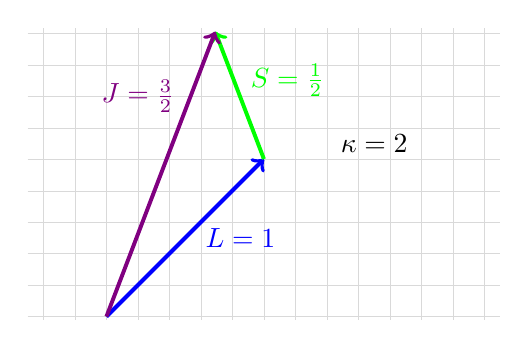
\begin{tikzpicture}[ thick,scale=2]
		% (IEI-B-1)
	\draw[gray!30,line width=0.01mm,step=0.2] (-0.5,-0.02) grid (2.5, 1.834);
	\draw[->,blue,line width=.5mm] (0, 0) -- (1, 1);
	\draw[->,green,line width=.5mm] (1, 1) -- (0.691, 1.809);
	\draw[->,violet,line width=.5mm] (0, 0) -- (0.691, 1.809);

	\node at (1.15,1.5) {\textcolor{green}{ $S=\frac{1}{2}$}};
	\node at (0.85,0.5) {\textcolor{blue}{ $L=1$}};
	\node at (0.2,1.4) {\textcolor{violet}{ $J=\frac{3}{2}$}};

	\node at (1.7,1.1) {\textcolor{black}{ $\kappa=2$}};
	
\end{tikzpicture}\qquad
\end{document}
